\documentclass[11pt, oneside]{article}   	% use "amsart" instead of "article" for AMSLaTeX format
\usepackage{geometry}                		% See geometry.pdf to learn the layout options. There are lots.
\geometry{letterpaper}                   		% ... or a4paper or a5paper or ... 
%\geometry{landscape}                		% Activate for for rotated page geometry
%\usepackage[parfill]{parskip}    		% Activate to begin paragraphs with an empty line rather than an indent
\usepackage{graphicx}				% Use pdf, png, jpg, or eps� with pdflatex; use eps in DVI mode
								% TeX will automatically convert eps --> pdf in pdflatex		
\usepackage{amssymb}
\graphicspath{{/Users/telliott_admin/Dropbox/Tex/png/}}

\title{Gaussian (normal) distribution:  derivation}
%\author{The Author}
\date{}							% Activate to display a given date or no date

\begin{document}
\maketitle
%\section{}
%\subsection{}
I'm going show a derivation of the Gaussian distribution from first principles.  The argument is originally due to Sir John F. W. Herschel.

Imagine that you are throwing darts at the origin of the x,y plane. Under perfect conditions, you would hit the center dead on every time. However, conditions aren't perfect. The wind is gusting, the music is loud, there are other distractions. As a result, small errors creep in and the pattern over time looks like so:

\begin{center}
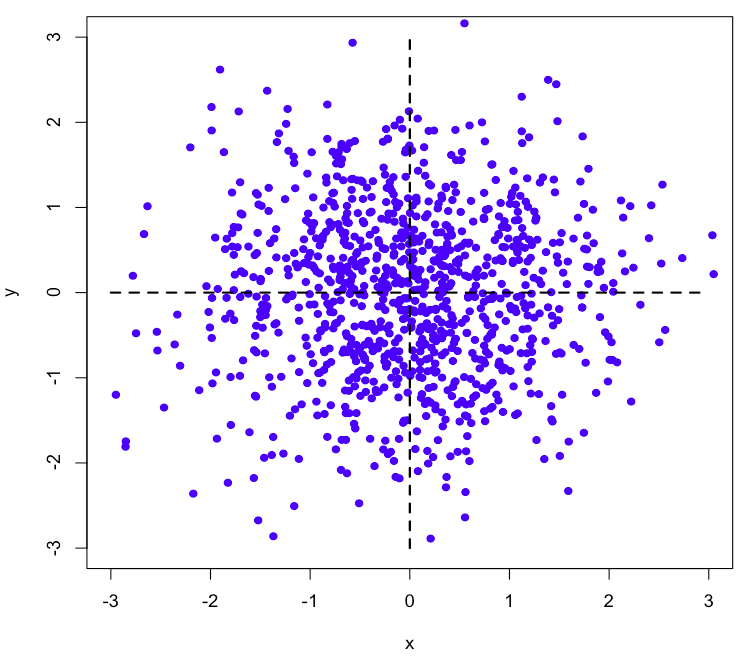
\includegraphics [scale=0.4] {gauss1.png}
\end{center}

Now, there is some unknown function for the probability that a dart will land in the interval between $x$ and $x + \Delta x$. Obviously, the probability depends on $x$, with a maximum at $x = 0$ and then decreasing to zero as $x$ gets large. We designate that function as a probability density function $p(x)$ and evaluate the density over the interval to get the probability that the dart lands in the interval:

\begin{center}
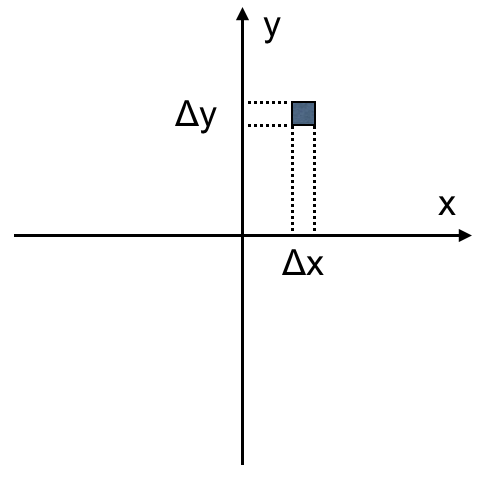
\includegraphics [scale=0.4] {gauss2.png}
\end{center}

\[ P = p(x) \Delta x \]

Now we consider a small area of size $\Delta x \Delta y$. If the errors in perpendicular directions are independent, then we expect that $p(x) = p(y)$ and we can get the probability that a dart lands in the small rectangle bounded by $x$, $y$ and $x + \Delta x$, $y + \Delta y$ as:

\[ P = p(x) \Delta x \ p(y) \Delta y\]

In fact, if we assume that the errors do not depend on the orientation of the coordinate system, then the probability is a function only of $r$, the radial distance from the origin, so we can write

\[ P = g(r) \Delta x \ \Delta y \]
\[ g(r) \Delta x \ \Delta y = p(x) \Delta x \ p(y) \Delta y \]
\[ g(r) = p(x)  \ p(y) \]

This assumption of rotational independence leads directly to the answer, as you will see. As Hamming says, since $r$ does not depend on the angle $\theta$, (but $x$ and $y$ do), we can take the partial derivative with respect to $\theta$ of $g(r)$ and set it equal to zero, so that:

\[ \frac{\partial g(r)}{\partial \theta} = 0 = p(x) \frac{\partial p(y)}{\partial \theta}  + p(y) \frac{\partial p(x)}{\partial \theta} \]

What are these derivatives?
\[ x = r \ cos \theta \]
\[ y = r \ sin \theta \]

\[ \frac{\partial p(x)}{\partial \theta} = \frac{\partial p(x)}{\partial x} \frac{\partial x}{\partial \theta}\]
\[ \frac{\partial x}{\partial \theta} = - r sin \theta \]
\[ \frac{\partial p(x)}{\partial \theta} = p'(x)(-y) \]

\[ \frac{\partial p(y)}{\partial \theta} = \frac{\partial p(y)}{\partial y} \frac{\partial y}{\partial \theta}\]
\[ \frac{\partial y}{\partial \theta} = r cos \theta \]
\[ \frac{\partial p(y)}{\partial \theta} = p'(y)(x) \]
This gives
\[ p(x)p'(y)(x) - p(y)p'(x)(y) = 0 \]
\[ \frac{p'(x)}{p(x)(x)} = \frac{p'(y)}{p(y)(y)} = K \]

What function do we know that has itself as the derivative (since $p'(x) = k p(x) $?
\[ p(x) = A e^{Kx^2/2} \]
\[ p'(x) = AK(x) e^{Kx^2/2} = K(x)p(x) \]
Since we assume that large errors are less likely than small ones, $K < 0$, so we can define another constant $V = - 1/K$ and
\[ p(x) = A e^{-x^2/2V} \]
This is the normal distribution with variance V.

It is amazing how far we got with this argument! We assumed:
(1) the errors do not depend on the orientation of the coordinate system.
(2) errors in perpendicular directions are independent. This means that being too high doesn't alter the probability of being off to the right.
(3) large errors are less likely than small errors.

Notice that although we started talking about a probability distribution in two dimensions, the function we end up with is for one dimension.

James Clerk Maxwell used the same argument in three dimensions to derive his expression for the distribution of molecular velocities in a gas.
\end{document}  